\section{Auditing and re-scoring existing benchmarks}
\label{sec:audit}

\paragraph{How guessable are the benchmarks?} Table~\ref{tab:audit} gives the reader's expected closed-book accuracy in
two ways: under prompts that ask for a best guess (mean over six draws of Qwen3-235B), which measures what the reader
knows, and under the evaluation prompt with an empty memory (three draws), which is what enters a score
(\S\ref{sec:procedure}). The second is clearly lower on the two conversational benchmarks, where the reader often abstains
when its memory is empty, and about the same on the document tasks. The last column, the share of items answered
correctly in at least one of seven guessing draws (six Qwen, one Llama-3.3-70B), grows with the number of draws (on LoCoMo
from \singleLocomo{} with one draw to \everLocomo{} with seven), so it is only a lower bound on what a determined reader
could guess.

\begin{table}[t]
\centering\small
\begin{tabular}{@{}lccc@{}}
\toprule
& \multicolumn{2}{c}{mean $\hat g$} & \\
\cmidrule(lr){2-3}
Benchmark (answerable items) & guess & eval. & ever \\
\midrule
LongMemEval & \gLme & \gEvalLme & \everLme \\
LoCoMo cat.\ 1--4 & \gLocomo & \gEvalLocomo & \everLocomo \\
MAB RULER-QA1 & \gQaOne & \gEvalQaOne & \everQaOne \\
MAB RULER-QA2 & \gQaTwo & \gEvalQaTwo & \everQaTwo \\
MAB EventQA & \gEventqa & \gEvalEventqa & -- \\
MAB FactConsolidation-SH & \gFcSh & \gEvalFcSh & -- \\
MAB FactConsolidation-MH & \gFcMh & \gEvalFcMh & -- \\
\bottomrule
\end{tabular}
\caption{Closed-book guessability of agent-memory benchmarks for the reader used in our re-scoring (MAB:
MemoryAgentBench). guess: prompts that ask for a best guess; eval.: the evaluation prompt with an empty memory; ever:
correct in at least one of seven guessing draws.}
\label{tab:audit}
\end{table}

\paragraph{Re-scoring twelve systems.} We ran twelve memory systems end to end on LoCoMo and on MemoryAgentBench
RULER-QA1, with a second document (QA2) as an independent replication: four libraries with their default prompts
(Mem0 2.2.1 and 1.0.11, LangMem, LlamaIndex fact extraction), the verbatim compaction prompts of five coding agents and
an LLM API (Codex, OpenHands, Aider, Gemini CLI, LangChain summarisation, Anthropic API), a neutral rewrite operator, and
raw retrieval. All share one reader (Qwen3-235B, $T{=}0$) and one judge. Contexts were saved so that every answer could
be re-asked under each protocol (Table~\ref{tab:protocols}). For systems that keep a single rewritten memory the reader
sees all of it; for Mem0 and raw retrieval it sees what the system retrieves for the question, so a low \cpr{} can reflect
a failure to write, keep or retrieve the fact. The analyses below were registered before we moved \cpr{} to $\pi_F$
(Appendix~\ref{app:deviations}) and use \cpr{} under $\pi_A$, except the ranking comparison, which pairs each protocol's
accuracy with its own \cpr{}; Table~\ref{tab:protocols} gives both versions.

\begin{table*}[t]
\centering\small
\begin{tabular}{l cccc cccc}
\toprule
& \multicolumn{4}{c}{LoCoMo (cat.\ 1--4, $n{=}1540$)} & \multicolumn{4}{c}{MemoryAgentBench RULER-QA1 ($n{=}100$)} \\
\cmidrule(lr){2-5}\cmidrule(lr){6-9}
System & Acc$_A$ & Acc$_F$ & CPR & Abst$_A$ & Acc$_A$ & Acc$_F$ & CPR & Abst$_A$ \\
\midrule
Raw RAG & 0.59 & 0.59 & 0.51 & 0.12 & 0.49 & 0.52 & 0.41 & 0.37 \\
Mem0 (2.2.1) & 0.41 & 0.42 & 0.33 & 0.24 & 0.77 & 0.77 & 0.70 & 0.11 \\
LangMem & 0.35 & 0.36 & 0.28 & 0.33 & -- & -- & -- & -- \\
LlamaIndex facts & 0.29 & 0.31 & 0.25 & 0.38 & 0.19 & 0.42 & 0.07 & 0.67 \\
Mem0 (1.0.11) & 0.21 & 0.22 & 0.16 & 0.47 & 0.35 & 0.32 & 0.00 & 0.20 \\
Gemini CLI & 0.18 & 0.19 & 0.14 & 0.52 & 0.18 & 0.29 & 0.00 & 0.67 \\
Neutral rewrite & 0.15 & 0.17 & 0.11 & 0.58 & 0.25 & 0.35 & 0.04 & 0.53 \\
OpenHands & 0.09 & 0.12 & 0.06 & 0.63 & 0.18 & 0.26 & 0.00 & 0.62 \\
LangChain summ. & 0.09 & 0.12 & 0.06 & 0.64 & 0.21 & 0.33 & 0.00 & 0.63 \\
Aider & 0.08 & 0.11 & 0.06 & 0.73 & 0.15 & 0.35 & 0.00 & 0.78 \\
Anthropic API & 0.07 & 0.10 & 0.04 & 0.70 & 0.24 & 0.30 & 0.00 & 0.55 \\
Codex & 0.07 & 0.10 & 0.04 & 0.62 & 0.15 & 0.28 & 0.00 & 0.78 \\
\bottomrule
\end{tabular}
\caption{Twelve memory systems re-scored with the same reader (Qwen3-235B) and judge. Acc$_A$/Acc$_F$: accuracy under the native
and the forced answer protocol; CPR: accuracy on prior-resistant items (native protocol); Abst$_A$: abstention rate on answerable
items under the native protocol (LLM-classified). LangMem fails on MemoryAgentBench documents (see \S\ref{sec:audit}).}
\label{tab:protocols}
\end{table*}


\paragraph{Abstention, not memory, drives raw-score differences among memory-poor systems.} On RULER-QA1,
\nPoorQaOne{} of \nSysQaOne{} systems answer at most 5\% of the resistant items under either protocol, yet their raw accuracies differ widely.
Their native-protocol abstention rate on answerable items ranges from \absRangeLo{} to \absRangeHi{}, and forcing an
answer raises accuracy most for the systems that abstain most (Figure~\ref{fig:abstention}): Spearman $\rho=\hOneQaOne$
[\hOneQaOneLo, \hOneQaOneHi] on QA1, $\hOneQaTwo$ on QA2 and $\hOneLocomo$ on LoCoMo (pre-registered primary test, Holm
corrected). Aider's accuracy, for instance, moves from \aiderAccA{} to \aiderAccF{} with no change in its memory. In
other words, a fixed backbone does not cancel the prior: the prior enters each system's score in proportion to its
willingness to guess. How much this matters depends on how guessable the benchmark is: forcing an answer changes a
system's accuracy by at most \gainMaxLocomo{} on LoCoMo but by up to \gainMaxQaOne{} on RULER-QA1.

\begin{figure}[t]
\centering
\definecolor{famA}{RGB}{0,114,178}
\definecolor{famB}{RGB}{213,94,0}
\definecolor{famC}{RGB}{0,158,115}
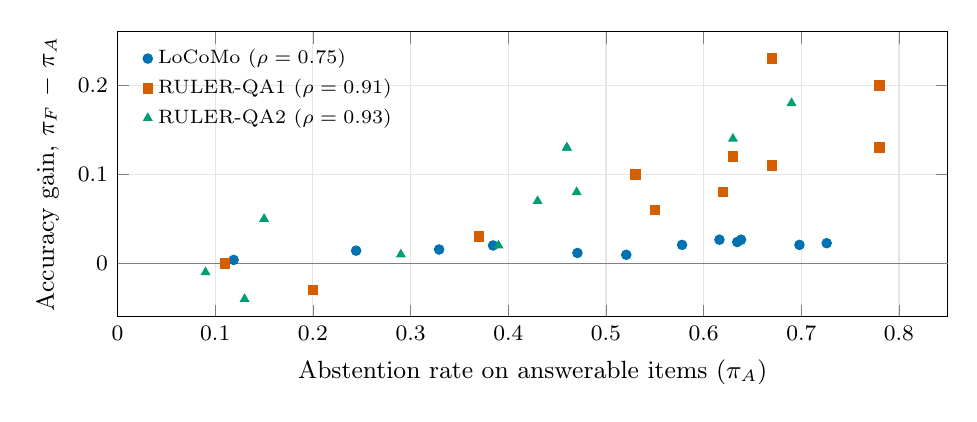
\begin{tikzpicture}
\begin{axis}[width=\columnwidth, height=5.2cm, xmin=0, xmax=0.85, ymin=-0.06, ymax=0.26,
  xlabel={Abstention rate on answerable items ($\pi_A$)}, ylabel={Accuracy gain, $\pi_F$ $-$ $\pi_A$},
  label style={font=\small}, tick label style={font=\footnotesize},
  legend style={font=\scriptsize, at={(0.02,0.98)}, anchor=north west, draw=none, fill=none},
  legend cell align=left, grid=major, grid style={gray!20}]
\addplot[gray, domain=0:0.85, forget plot] {0};
\addplot[only marks, mark=*, mark size=1.7pt, draw=famA, fill=famA] coordinates {(0.7260,0.0227) (0.6981,0.0208) (0.6162,0.0266) (0.5208,0.0097) (0.6383,0.0266) (0.3292,0.0156) (0.3844,0.0201) (0.2442,0.0143) (0.4708,0.0117) (0.5779,0.0208) (0.6344,0.0240) (0.1188,0.0039)};
\addlegendentry{LoCoMo ($\rho=0.75$)}
\addplot[only marks, mark=square*, mark size=1.7pt, draw=famB, fill=famB] coordinates {(0.7800,0.2000) (0.5500,0.0600) (0.7800,0.1300) (0.6700,0.1100) (0.6300,0.1200) (0.6700,0.2300) (0.1100,0.0000) (0.2000,-0.0300) (0.5300,0.1000) (0.6200,0.0800) (0.3700,0.0300)};
\addlegendentry{RULER-QA1 ($\rho=0.91$)}
\addplot[only marks, mark=triangle*, mark size=1.7pt, draw=famC, fill=famC] coordinates {(0.4600,0.1300) (0.4300,0.0700) (0.6300,0.1400) (0.4600,0.1300) (0.2900,0.0100) (0.6900,0.1800) (0.0900,-0.0100) (0.1300,-0.0400) (0.3900,0.0200) (0.4700,0.0800) (0.1500,0.0500)};
\addlegendentry{RULER-QA2 ($\rho=0.93$)}
\end{axis}
\end{tikzpicture}

\caption{Forcing an answer helps most the systems that abstain most. Each point is one memory system
on one benchmark (same reader and judge throughout); $\rho$ is the pre-registered Spearman correlation between
abstention under the native protocol and the accuracy gained by forcing an answer.}
\label{fig:abstention}
\end{figure}

\paragraph{Standardising the protocol does not recover memory rankings.} We predicted that under $\pi_F$ raw accuracy
would rank systems more like \cpr{} does. It did not (change in Kendall $\tau$: $\dtauQaOne$ [\dtauQaOneLo, \dtauQaOneHi]
on QA1, $\dtauQaTwo$ on QA2). An exploratory reading: forcing an answer pushes all memory-poor systems toward the guess
rate, so they tie, and their order becomes noise. Protocol standardisation removes the abstention confound but does
not separate memory from guessing; that requires the prior split. We also find no pairwise rank reversal that is
statistically confirmed in both directions (\confirmedRev{} pairs), so our claims rest on inflation and confounding,
not on reversed leaderboards.

\paragraph{Scoring unanswerable items rewards forgetting.} We pose LoCoMo's unanswerable (category-5) questions as open
questions, like the other categories, and judge them with LongMemEval's abstention prompt; the original LoCoMo harness
instead offers two options, one of which is ``Not mentioned in the conversation'', so that chance is 50\%. In this category, a system's rate of correct
abstention is negatively related to its \cpr{} across the twelve systems ($\rho=\rhoCaCpr$; raw category accuracy:
$\rho=\rhoRawCatFive$): the less a system remembers, the more readily it says the information is missing. Scoring
discrimination instead ($J$) reverses the sign ($\rho=\rhoJCpr$).

\paragraph{Is the inflation an artefact of aggressive compaction?} Our harness compacts after every ingested chunk,
which is far more often than products do. Re-running the seven compaction systems with a realistic trigger (compact
only when the live context exceeds 64k tokens) raises their \cpr{} on QA1 from near zero to
\thrCprMin--\thrCprMax{}, so the near-empty memories are partly a property of the stress protocol. The prior inflation
persists, however: the gap between prior-answerable and resistant accuracy remains positive with a confidence interval
excluding zero in \inflPairs{} of 14 system--document pairs, and the abstention effect holds under both triggers.
